% Created 2023-09-15 vie 00:11
% Intended LaTeX compiler: pdflatex
\documentclass[11pt]{article}
\usepackage[utf8]{inputenc}
\usepackage[T1]{fontenc}
\usepackage{graphicx}
\usepackage{grffile}
\usepackage{longtable}
\usepackage{wrapfig}
\usepackage{rotating}
\usepackage[normalem]{ulem}
\usepackage{amsmath}
\usepackage{textcomp}
\usepackage{amssymb}
\usepackage{capt-of}
\usepackage{hyperref}
\usepackage{../modern}
\bibliography{./fuentes.bib}
\raggedbottom
\setcounter{secnumdepth}{2}
\author{Luis Eduardo Galindo Amaya (1274895)}
\date{12 de Septiembre 2023}
\title{Taller 1 Sistema de Archivos}
\hypersetup{
 pdfauthor={Luis Eduardo Galindo Amaya (1274895)},
 pdftitle={Taller 1 Sistema de Archivos},
 pdfkeywords={},
 pdfsubject={},
 pdfcreator={Emacs 27.1 (Org mode 9.3)}, 
 pdflang={Spanish}}
\begin{document}

\modentitlepage{../images/escudo-uabc-2022-color-cont.png}
\tableofcontents\pagebreak
\datasection{Individual}


\section{Introducción}
\label{sec:org0ee8b52}
Los sistemas Unix o Unix-Like siempre se han caracterizado por tener una 
cantidad de software amplia la cual permite contruir utilidades muy poderosas,
durante el taller se estudiara como crear, modificar, eliminar y ver los detalles
de archivos del sistema.   

\section{Actividades}
\label{sec:org865ee98}
\subsection{Despliegue el nombre del directorio de trabajo actual}
\label{sec:org76c2fcd}
\begin{verbatim}
pwd
\end{verbatim}

\begin{figure}[htbp]
\centering
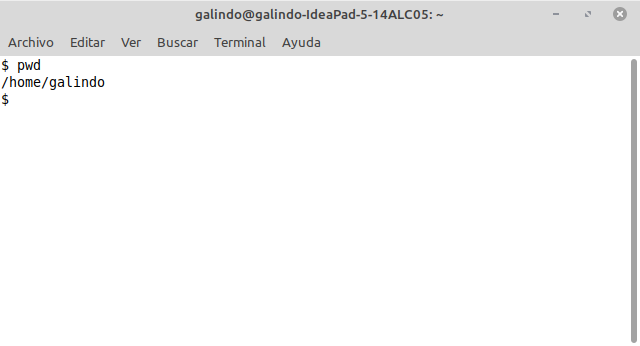
\includegraphics[width=10cm]{img/1.png}
\caption[\texttt{pwd}]{Salida del comando \texttt{pwd}}
\end{figure}

\subsection{Lista en forma de columnas (sin detalles) el contenido del directorio padre de su home directory}
\label{sec:orgc7201d5}
\begin{verbatim}
ls -1
\end{verbatim}

\begin{figure}[htbp]
\centering
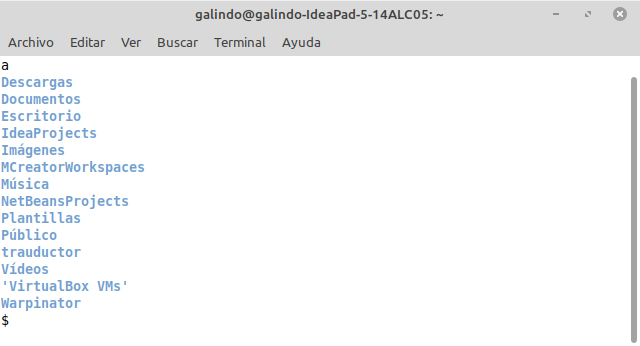
\includegraphics[width=10cm]{img/2.png}
\caption{El flag -1 muestra los archivos como columna}
\end{figure}

\cite{AskUbuntu_2017}

\subsection{Lista en orden alfabético inverso todos los archivos (incluyendo los ocultos) de su home directory.}
\label{sec:orgebaee46}
\begin{verbatim}
ls -r -A ~
\end{verbatim}

\begin{figure}[htbp]
\centering
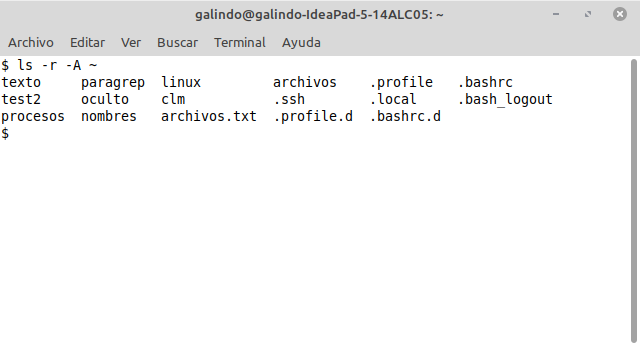
\includegraphics[width=10cm]{img/3.png}
\caption[\texttt{-A}]{\texttt{-r} invierte el orden y \texttt{-A} muetra todos los archivos}
\end{figure}

\pagebreak

\subsection{Lista en orden alfabético el contenido de su home directory mostrando información detallada.}
\label{sec:org2dfd41e}
\begin{verbatim}
ls -l
\end{verbatim}

\begin{figure}[htbp]
\centering
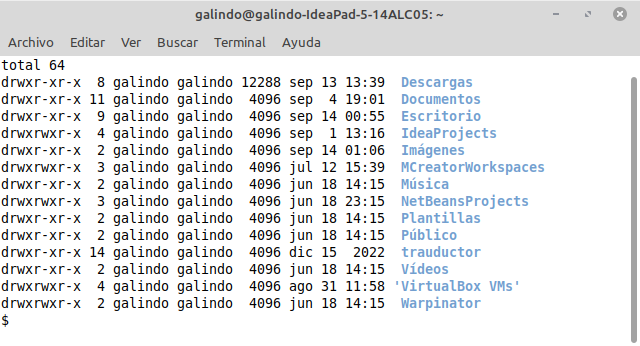
\includegraphics[width=10cm]{img/4.png}
\caption[\texttt{-l}]{\texttt{-l} agrega todos los detalles sobre un archivo, creador y fecha}
\end{figure}

\subsubsection*{¿En qué consiste esa información?}
\label{sec:org98c6156}
\begin{mdframed}
La información mostrada contiene los permisos, el creador, el peso del archivo, ultima modificación y nombre de los archivos
\end{mdframed}

\subsubsection*{¿Qué significa el primer carácter que se muestra en la lista?}
\label{sec:org4c80872}
\begin{mdframed}
Si el archivo es un directorio, si el carácter es 'd' es directorio si no entonces es un archivo
\end{mdframed}

\subsection{Desarrolle la estructura de directorios que se indique en el pizarrón.}
\label{sec:orga4bc970}

\begin{figure}[htbp]
\centering
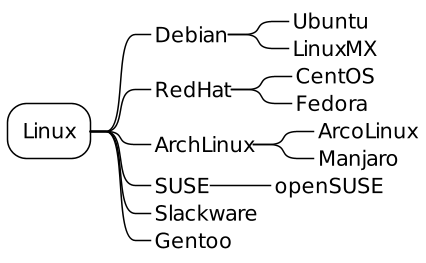
\includegraphics[width=6cm]{./img/tree.png}
\caption{Árbol de directorios}
\end{figure}

\begin{verbatim}
mkdir Linux
cd Linux
mkdir -p Debian/Ubuntu Debian/LinuxMX
mkdir -p Redhat/CentOS Redhat/Fedora
mkdir -p ArchLinux/ArcoLinux ArchLinux/Manjaro
mkdir -p SUSE/openSUSE
mkdir Slackware Gentoo
\end{verbatim}

\autocite{TecAdmin_2023}

\subsection{Verifique que la estructura haya sido creada correctamente.}
\label{sec:org71a2a75}
\begin{verbatim}
ls -R
\end{verbatim}

\begin{figure}[htbp]
\centering
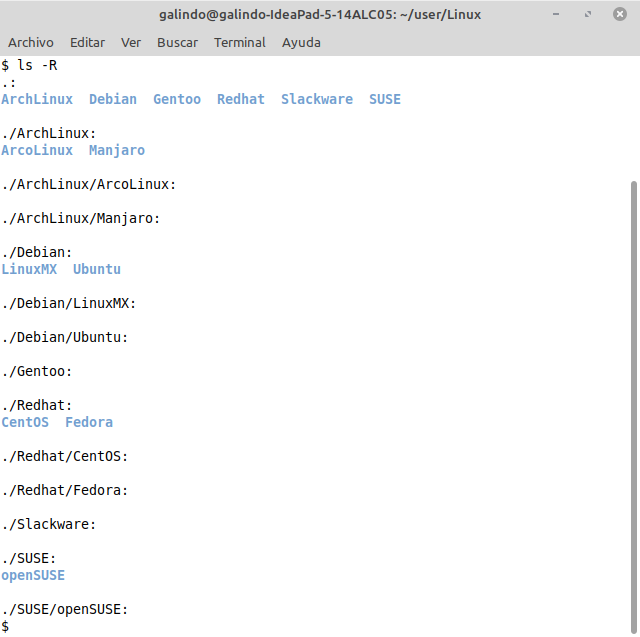
\includegraphics[width=10cm]{img/6b.png}
\caption[\texttt{-R}]{\texttt{-R} muestra el arbol de directorios creados}
\end{figure}

\subsection{Borre el último nivel del árbol de directorios.}
\label{sec:org4a289af}
\begin{verbatim}
rm -r Debian/Ubuntu Debian/LinuxMX
rm -r Redhat/CentOS Redhat/Fedora
rm -r ArchLinux/ArcoLinux ArchLinux/Manjaro
rm -r SUSE/openSUSE
\end{verbatim}

\begin{figure}[htbp]
\centering
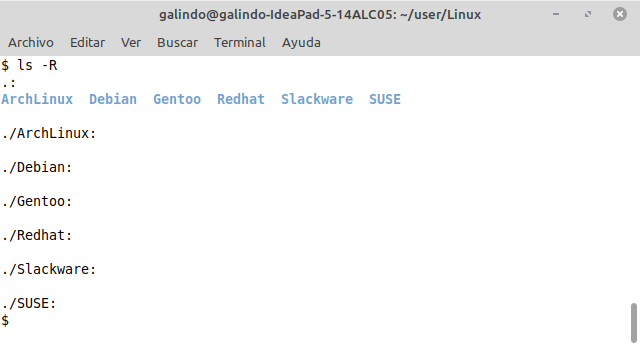
\includegraphics[width=9.5cm]{img/7.png}
\caption{Eliminado uno a uno los últimos nodos del árbol}
\end{figure}

\begin{figure}[htbp]
\centering
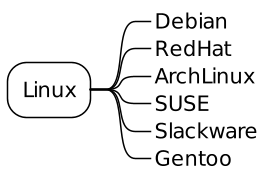
\includegraphics[width=5cm]{./img/tree2.png}
\caption{Árbol de directorios resultante}
\end{figure}

\pagebreak

\subsection{Lista el contenido de su directorio, mostrando de forma simbólica el tipo de archivos que contiene.}
\label{sec:org4788de0}
\begin{verbatim}
ls -F
\end{verbatim}

\begin{figure}[htbp]
\centering
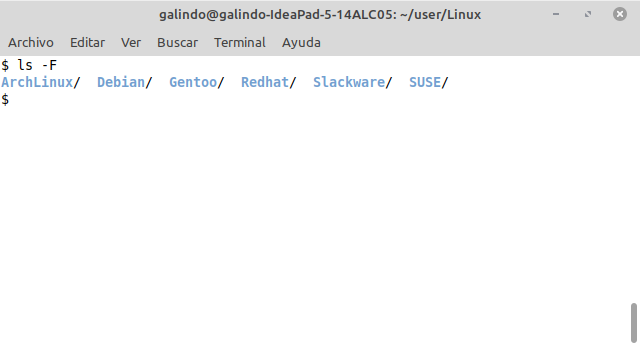
\includegraphics[width=10cm]{img/8.png}
\caption{\texttt{-F} muestra el tipo simbólico '/' si es directorio y vació si es archivo}
\end{figure}

\pagebreak

\subsection{¿Para qué sirve el comando \texttt{whoami}?}
\label{sec:org96f95e2}
\begin{mdframed}
Mostrar el nombre de usuario efectivo
\end{mdframed}
\cite{linux_whoami} 

\subsection{¿Qué información nos proporciona \texttt{uname}?}
\label{sec:org496129e}
\begin{mdframed}
Imprime el nombre del sistema operativo
\end{mdframed}
\cite{OpenBSD_uname}

\subsection{Dentro de un directorio llamado alumnos, cree un directorio para cada alumno del salón, asignándole como nombre el user name de cada persona (verifique la lista de usuarios mediante el comando \texttt{who})}
\label{sec:orga3cf306}
\begin{verbatim}
mkdir alumnos
cd alumnos 

mkdir richelle brenda galindo axl pelayo luis99 gerardo\
      arriaga pepeam roger emmanuel hector ruben nicole\
      alan
\end{verbatim}

\begin{figure}[htbp]
\centering
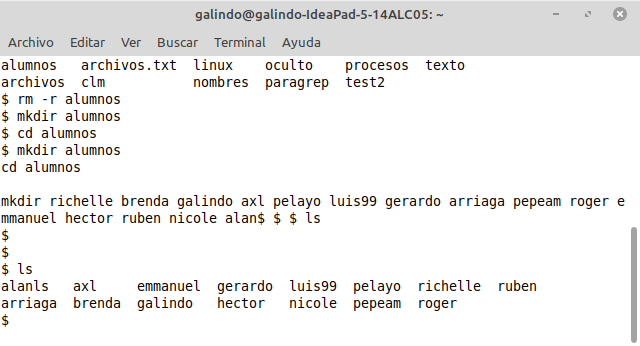
\includegraphics[width=10cm]{img/11.png}
\caption{Directorios creados}
\end{figure}

\subsection{Renombre todos los directorios del directorio alumnos con los nombre reales de sus compañeros.}
\label{sec:org536b65f}
\begin{verbatim}
mv richelle/ RICHELLE_NADINE_REYES_UDASCO/
mv brenda/ BERNARDO_MORALES_RAMOS/
mv galindo/ LUIS_EDUARDO_GALINDO_AMAYA/
mv axl/ AXEL_GOMEZ_BETANCOURT/
mv pelayo/ ALAN_ALEXANDER_PELAYO_FRIAS/
mv luis99/ LUIS_FELIPE_RODRIGUEZ_RODRIGUEZ/
mv gerardo/ GERARDO_ANTONIO_ABDALA_LOPEZ/
mv arriaga/ RENE_SEBASTIÁN_ARRIAGA_ALONSO/
mv pepeam/ JOSÉ_ANTONIO_ARCE_MONTOYA/
mv roger/ ALAN_ROGELIO_MARTINEZ_SIFUENTES/
mv emmanuel/ EMANUEL_CASTRO_VEGA/
mv hector/ HÉCTOR_MIGUEL_MACÍAS_BALTAZAR/
mv ruben/ RUBEN_STELLIOS_RUIZ_ALONSO/
mv nicole/ NICOLE_SOFÍA_ORTIZ_LOPEZ/
mv alan/ ALAN_FERNANDO_LEÓN_CORTEZ/
\end{verbatim}


\begin{figure}[htbp]
\centering
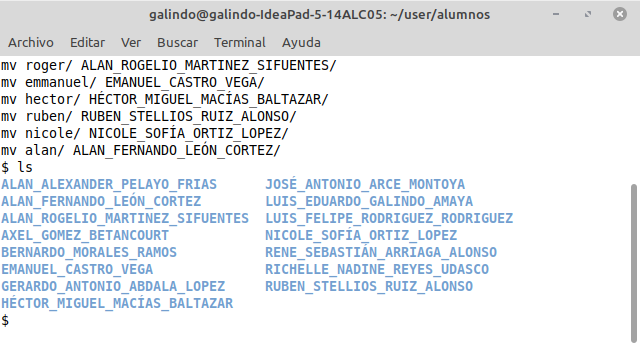
\includegraphics[width=10cm]{img/12.png}
\caption[\texttt{mv}]{\texttt{mv} permite mover archivos o renombrarlos}
\end{figure}

\subsection{Liste los directorios en forma alfabética}
\label{sec:org312f3bc}
\subsubsection*{¿Quién es el dueño de los directorios creados? ¿Cúal es la fecha de creación?}
\label{sec:orgfa369e3}
\begin{mdframed}
Para conocer la información del dueño y la fecha de creación se puede usar el
comando \texttt{ls -l} y examinar las columnas de dueño y fecha de creación 
\end{mdframed}

\begin{figure}[htbp]
\centering
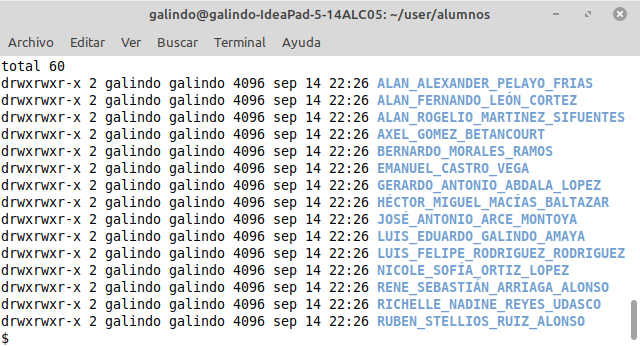
\includegraphics[width=10cm]{img/13a.png}
\caption[\texttt{ls}]{\texttt{ls} con detalles de los archivos}
\end{figure}

\subsection{Borre en un solo paso la estructura anterior. Auxiliese del manual de ayuda}
\label{sec:org6ebc893}
\begin{verbatim}
rm -r alumnos
\end{verbatim}

\begin{figure}[htbp]
\centering
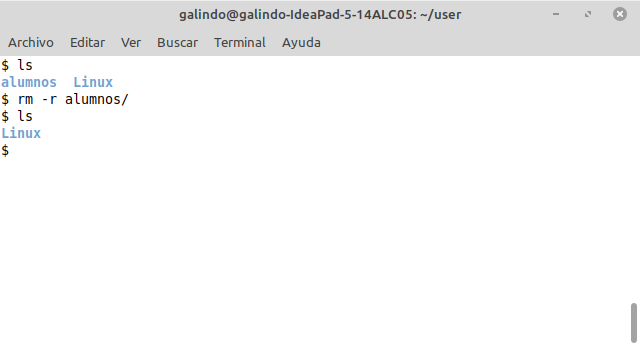
\includegraphics[width=10cm]{img/14.png}
\caption[\texttt{-r}]{\texttt{-r} Elimina recursivamente los directorios la interior}
\end{figure}

\section{Conclusión}
\label{sec:org1dceee5}
A lo largo de esta practica pude entender como crear directorios, listarlos
modificarlos pude crear secuencias que hacen muchas cosas, pienso yo que 
al combinar estos comandos entre si seria posible crear aplicaciones completas 
que me pueden ayudar a cumplir tareas de administración. 

\pagebreak

\section{Referencias}
\label{sec:orgdc9faa2}
\printbibliography[heading=none]
\end{document}
